% file to contain information on examples
%==============================================================================
\chapter{Examples Explained - WIP}
Examples are located in the \verb|0-examples| folder and are designed to be run in batch mode.
This means that each example copies any required system, model, or modulation file to the main PST directory before running.
Typically, each example folder contains a \verb|.m| file that starts with \verb|run| that can be used to run the example.
As example cases are located on a github repository, relative file paths are used so that examples can be run without much difficulty from various different machines.
While most examples can be run in multiple versions of PST, some functionality can only be found in specific versions.

\noindent The general structure of created examples tend to reflect the following:
\begin{enumerate}
\itemsep 0em
\item Clear all variables, close all figures, and clear the command window
\item Define which version of PST to use
\item Create a relative path to the root directory of chosen PST version
\item Copy any system, model, or modulation file to the PST root directory
\item Run \verb|s_simu|
\item Save output data
\item Restore any model, or modulation file to original state
\item Create data plots
\end{enumerate}

%=================================================================
\pagebreak
\section{Standard Faulting (hiskens)}
Standard PST simulations involve some kind of fault defined in the \verb|sw_con| array.
This example (located in the \verb|hiskens| folder) is included to showcase some simple differences between PST versions using a standard test case.
System data for this example comes from a report by Ian Hiskens \cite{hiskens2013} which summarized a study of an IEEE 10 generator, 39 bus system.
Ryan Elliott at Sandia National Labs recreated the system in a PST format and provided the data file for this project.
A one-line diagram of the system is shown in Figure \ref{fig: hiskens oneline}.

\begin{figure}[H]
	\centering
	\footnotesize
	\includegraphics[width=.85\linewidth]{figures/hiskens/hiskensOneline}
	\caption{IEEE 39 bus network.}
	\label{fig: hiskens oneline}
\end{figure}%\vspace{-1 em}

The simulated event was a 0.1 second three-phase fault with no loss of line between bus 2 and 3.
The \verb|run_datane_hiskens.m| file can be used to run the simulation.
Figure \ref{fig: hiskens results} shows the resulting fault bus voltage magnitude and system generator speeds.

\begin{figure}[H]
	\centering
	\footnotesize
	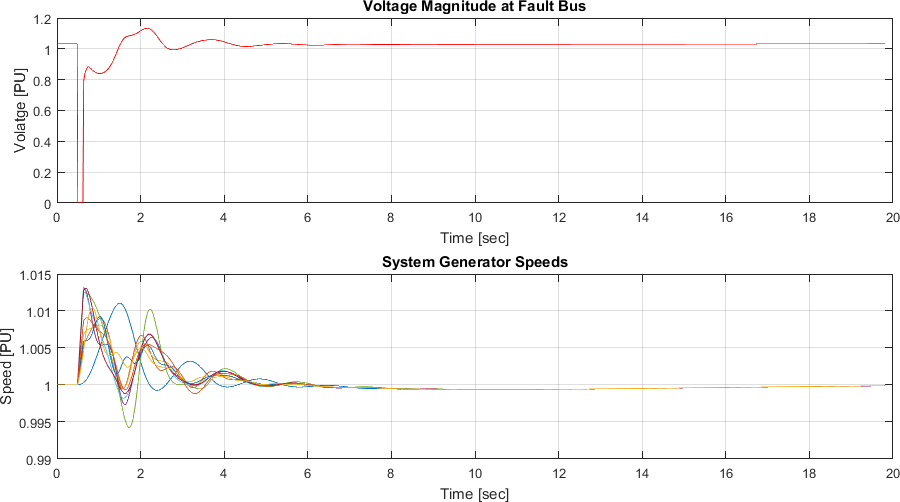
\includegraphics[width=\linewidth]{figures/hiskens/hiskensResults}
	\caption{Hiskens Example Fault Bus Voltage and Generator Speeds.}
	\label{fig: hiskens results}
\end{figure}%\vspace{-1 em}

All PST versions (when using the same models) provide the same results, but there are differences in simulation speed and data output.
Table \ref{tab: hiskens} shows that the PST 4 simulation was roughly twice as fast as PST version 2 or 3, saved less data, and left fewer variables in the MATLAB workspace post simulation.
These improvements are likely due to the restructuring of global variables and code to remove any `all zero` data from being saved.\\

% table data for hiskens fault comparison 


\begin{table}[H]
%\resizebox{\linewidth}{!}{ % Use to resize large tables
\singlespacing
	\begin{tabular}{@{} L{1.75cm} 
	R{2cm} R{2cm}  R{2cm} @{}} 	
		\toprule % @ signs to remove extra L R space
		\footnotesize % this will affect the table font (makse it 10pt)
		\raggedright % for non justified table text
						
										
										
		PST Version	&	Simulation Time [seconds]	&	Resulting Workspace Variables	&	Saved Data Size [KB]	\\ \midrule	
		2.3	&	16.56	&	206	&	7,549	\\	
		3.1	&	16.70	&	210	&	7,548	\\	
		SETO	&	8.42	&	24	&	3,965	\\	
		4	&	7.96	&	6	&	3,974	\\	\bottomrule

													
	\end{tabular}

	\caption{PST Version Comparisons of Hiskens Example.}
	\label{tab: hiskens}
%	}%end resize box
\end{table}






%=====================================================================
% all current examples
\pagebreak
All examples from 0-examples folder are listed below - last bit of User manual work will be to `thin the herd', insert previous results, confirm working, and provide minor details about content

Modulation files for PST version 2 and 3 assume input to function is (t, k), i.e. time vector and data index.


\section{AGC - WIP}
PST 4 only

run\_AGC- 2 area kundur with optional integration methods = load step - 120 second recovery.

 run\_AGC\_mod - same system as above - uses Interchange modulation signal as perturbance


\section{DC - WIP}
All versions - linear analysis doesn't seem to work, non-linear simulation seems to work

\section{exciterBatchTests - WIP}
PST 4 only - used to compare all 4 exciter models linear/non-linear response to load step

\section{extendedTerm - WIP}
Results written up in 200806-ExtendedVersionComp

\section{hiskens - WIP}
Basic tripping - covered in above section

\section{inductive - WIP}
meant to verify functionality of inductive generators and loads (motors)

Multiple cases run from example script: fault example and load pulse with linear/non-linear comparison.
Works in all versions.

\section{ivmmod - WIP}
example modified from Dan - includes a VTS example  -
requires some minor reworking - 

shows how angle change `moves' entire system.

\section{lmod - WIP}
Requires clean up - one of first example cases -- update to follow similar strucutre as newer examples.

\section{mexc - WIP}
Exciter signal modulation with linear/non-linear comparison

Works in all versions of PST

\section{miniWECC - WIP}
	miniWECC - examples pretty sloppy - trips of line / colstrip

	miniWECCAGC - 

	miniWECC-genTrip -


\section{mtg\_sig - WIP}
\section{OMIB - WIP}
\section{pm\_sig - WIP}
Modulation of mechanical power to a generator - linear/non-lienar comparison

Works in all versions

\section{pss  - WIP}
\section{pwrmod-Iinjection - WIP}

\section{pwrmod-Pinjection  - WIP}

\section{rlmod - WIP}
Reactive load modulation

linear/non-linear comparison plots

Works in all Versions

\section{SVC - WIP}
Modulation of Static Var Compensator

linear/non-linear comparison plots

Works in all versions

\section{TCSC - WIP}
Modulation of Thyristor Controlled Series Reactor...

linear/non-linear comparison plots

Works in all versions

\section{tg - WIP}
Simple load step - contains to run files: one with governors, one without

Plot of system machines speeds - meant to show how governors act to arrest frequency change.

Works in all versions


\section{untrip - WIP}
Documentation created in \verb|MT-Tech-SETO\researchDocs\TEX\one-offs\200901-refinedUntripResults2|

Variables to note in associated examples (where \verb|x| is the internal model number):
\begin{itemize}
\item exciter $V_{ref} = $ \verb|g.exc.exc_pot(x,3)|
\item governor $P_{ref} = $ \verb|g.tg.tg_pot(x,5)|
\item governor $\omega_{ref} = $ \verb|g.tg.tg_con(x,3)|
\end{itemize}